%%%%%%%%%%%%%%%%%%%%%%%%%%%%%%%%%%%%%%%%%%%%%%%%%%%%%%%%%%%%%%%%%
\chapter{INTRODUCTION}\label{introduction}
%%%%%%%%%%%%%%%%%%%%%%%%%%%%%%%%%%%%%%%%%%%%%%%%%%%%%%%%%%%%%%%%%


\section{Introduction to Nanofluids}

The fast pace of microprocessor technology, the invention of higher performance smaller processors, have risen a new challenge to cope with: thermal management. Cooling plays a vital role for many systems, not only electronic designs due to the lack of space in todays tiny components but also from efficiency perspective as in automative systems such as fuel efficiency thanks to the smaller heat exchangers by increasing heat transfer enabling lighter automobile designs. 

Heat flow is governed by three main variables; heat transfer coefficient, heat transfer area and temperature difference. Increasing any of them or some of them simultaneously results in an increase in the heat transfer. Increasing the heat transfer difference is mostly possible by reducing the temperature of the coolant since increasing the temperature of the system is controversial to the fact that the opposite, reducing temperature of the system, is the end goal. Most of the times a temperature decrease in the coolant is not very efficient to go through, yet used in many applications. Another approach is to maximize the heat transfer area as seen in heat exchangers but is mostly constrained by todays attitude toward miniaturization such as in microprocessors and microelectromechanical systems (MEMS) where the heat transfer area is strictly constrained or aerospace systems where it might increase the weight which is substantially undesired for this specific domain \cite{beck2008thermal}. 
Increasing heat transfer coefficient to enhance heat transfer is another viable option, which can be achieved either via efficient heat transfer methods or use of materials with superior properties, such as forced convection or adding some particles to the conventional heat transfer fluids to change their inherently poor characteristics.

The idea to add particles originates form the fact that metals in solid form have orders-of-magnitude higher thermal conductivities than those of fluids Fig. ~\ref{fig:thermalCondGeneral}. To give an idea, thermal conductivity of copper at room temperature is about 700 times greater than that of water and about 3000 times greater than that of engine oil. Also, the thermal conductivity of metallic liquid score over than that of non-metallic liquids. 

This supports the fact that solid metallic particle suspension would have higher thermal conductivities compared to conventional heat transfer fluids. This drove the researches to experiment on this idea especially on micro and larger sized particles since smaller ones were not yet readily available due to not yet delivered technologies. Originally, this idea has ancient roots, going back to Maxwell who worked on the topic more than 100 years ago. But then, solid particles were settling out of suspension fast since they were large in size and dense. Thus the lack of stability prevented their practical use in the real world problems. 

The evolved technology made it possible to design and produce particles of sizes much smaller as in Fig. ~\ref{fig:nanoLengthScaleEx}. Nanotechnology became a popular topic since then, with its applications on a wide variety of topics ranging from medicine to cosmetics. The nano world is really fascinating, the materials of that size possess unique chemical and      physical properties. 

Nano-sized particle suspensions are called nanofluids. Use of nanofluids has appeared as an innovative way to enhance heat transfer via suspensions of metallic nano-sized particles in conventional heat transfer fluids. 

\begin{figure}
% Use the relevant command to insert your figure file.
% For example, with the graphicx package use
 \centering
  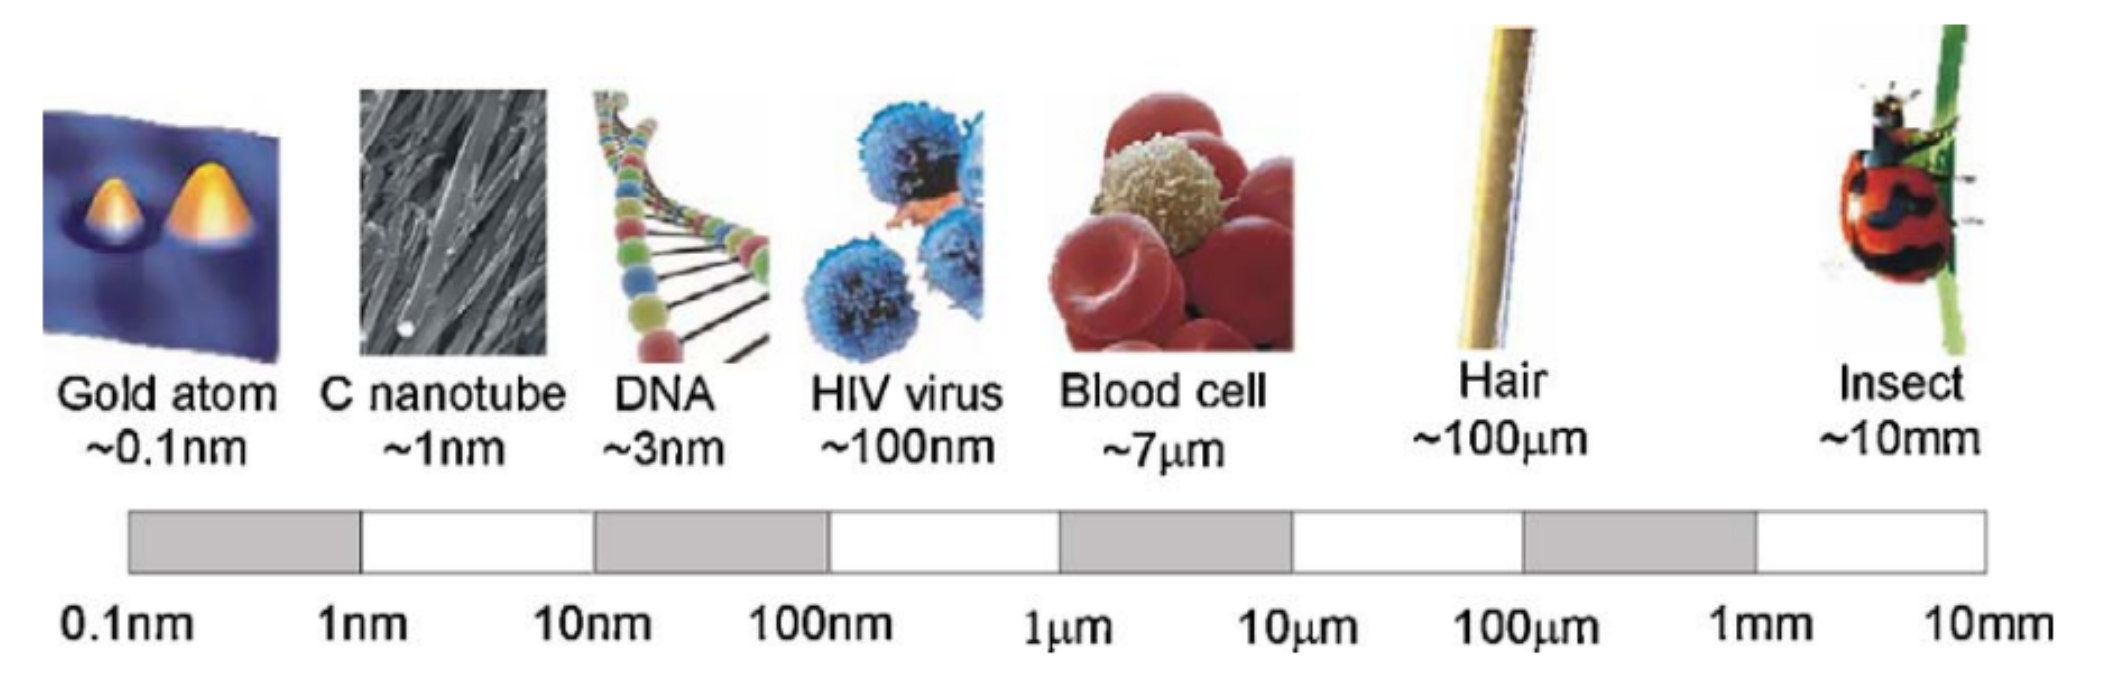
\includegraphics[scale=0.4]{figures/nanoLengthScaleEx}
% figure caption is below the figure
\vspace*{6mm}
\caption{Nano length scale examples \cite{serrano2009nanotechnology}.}
\label{fig:nanoLengthScaleEx}       % Give a unique label
\end{figure}

\begin{figure}
% Use the relevant command to insert your figure file.
% For example, with the graphicx package use
 \centering
  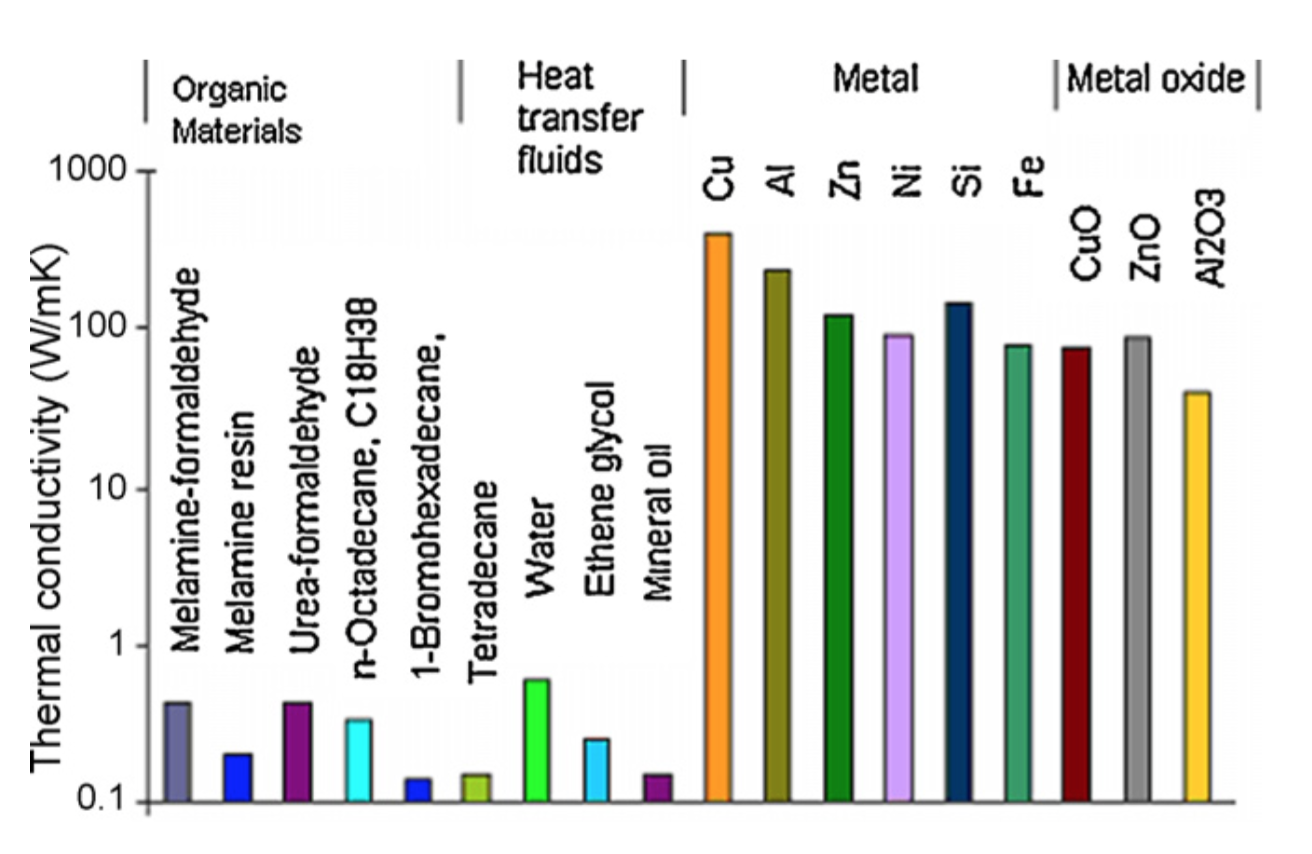
\includegraphics[scale=0.6]{figures/thermalCondGeneral}
% figure caption is below the figure
\vspace*{6mm}
\caption{Thermal conductivities of common liquids, polymers and solids \cite{wen2009review}.}
\label{fig:thermalCondGeneral}       % Give a unique label
\end{figure}


The technology advanced to a level where production of materials with an average crystallite size below 50 nm is possible. The term nanofluids, fluids with suspended nanoparticles, coined by Choi in 1995 in Argonne National Laboratory. Those next-generation heat transfer fluids offer exciting advantages over the conventional heat transfer fluids and also over the suspensions of micro-sized metallic particles. Increased surface area of the nanofluids results in enhanced heat transfer capabilities and the stability of the suspension is also improved. Aside those advantages about heat transfer, they are found to be better in terms of abrasion related properties. So now it seems to be obvious that clever use of those engineered fluids results in better designs such as smaller and light-weight heat exchanger systems. But literature seems to be not agreed upon the abilities of those fluids since there is a lack of agreement between the results of experiments and deserted theoretical understanding behind the mechanisms which govern nanofluids. 

The change in the size of the particles may result in different forces to dominate on the system and scaling theory is a tool to understand the most influential ones. As the size of the particles approach to nano scale, the effect of particle Brownian motion on the heat and mass transfer increases. The interaction force between the particles also becomes more evident compared to macro-sized particles where those are mostly neglected. So to deliver good designs, it is vital to identify the dominant mechanisms corresponding to the size scale of the system. 

Some of the advantages of nanofluids can be listed but not limited to \cite{choi1995enhancing}:

\begin{itemize} \item Increased specific surface area which results in increased heat transfer surface in-between particles and fluids \item  Increased stability in dispersion thanks to dominant Brownian motion \item Reduced pumping power in comparison to pure liquids to achieve same heat transfer intensification task \item  Reduced particle clogging \item  Adjustable properties via changing particle concentrations as in Fig. ~\ref{fig:thermalCondEnhancementChoi} and sometimes magnetic field and/or temperature as in Fig. ~\ref{fig:thermalCondComparison}\end{itemize}

\begin{figure}
% Use the relevant command to insert your figure file.
% For example, with the graphicx package use
 \centering
  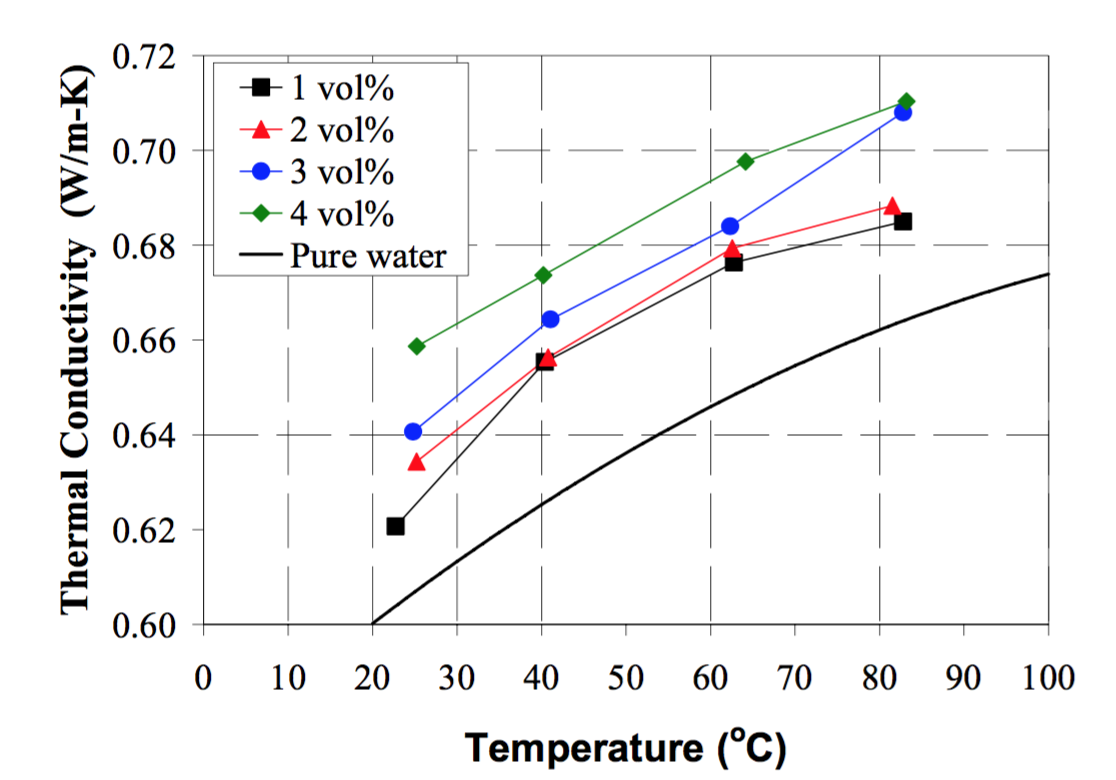
\includegraphics[scale=0.65]{figures/thermalCondComparison}
% figure caption is below the figure
\vspace*{6mm}
\caption{$Al_2O_3$ nanofluid temperature dependency on thermal conductivity\cite{shen2008minimum}.}
\label{fig:thermalCondComparison}       % Give a unique label
\end{figure}

\begin{figure}
% Use the relevant command to insert your figure file.
% For example, with the graphicx package use
 \centering
  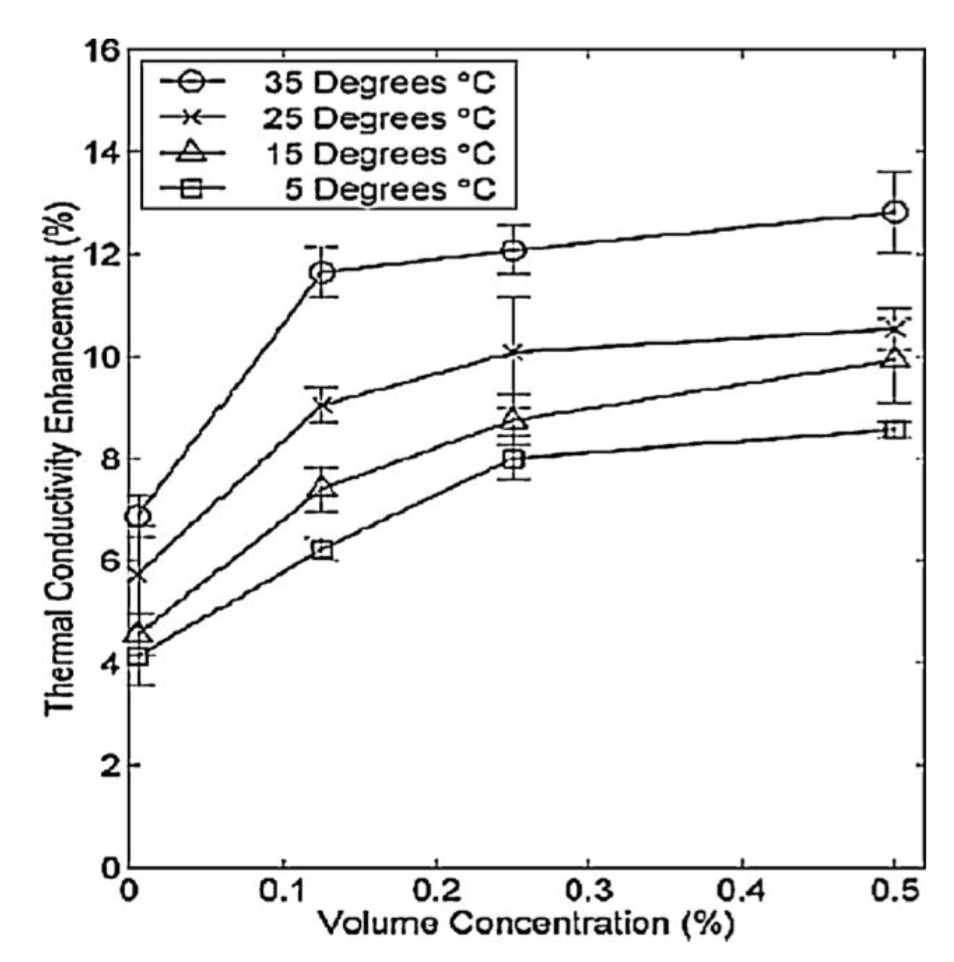
\includegraphics[scale=0.60]{figures/thermalCondEnhancementChoi}
% figure caption is below the figure
\vspace*{6mm}
\caption{Nanofluid thermal conductivity enhancement dependency on particle volume concentration in different temperatures  \cite{choiNanofluids}.}
\label{fig:thermalCondEnhancementChoi}       % Give a unique label
\end{figure}



\section{Literature Review}\label{literaturereview}


Currently, the cooling needs of cutting edge technologies pose a challenge to existing cooling fluids since they are actually poor conductors of heat. The chance of designing an enhanced, more conductive cooling fluid led some researchers to discover the strange world of the nano size. Nanofluids, engineered colloidal suspensions of nanoparticles (typically less than 100 nm) in a base fluid, usually~conventional cooling fluids, seem to be a new key to hurdle with the thermal bottleneck for various applications. Thus the research guided to these tiny particles as efficient tools to cope up with the thermal needs of not only small in size applications such as microelectromechanical systems (MEMS),
%Please define if possible
but also giant processes such as nuclear reactors.  The underlying mechanisms of the novel properties concerning nanofluids are still a mystery from the scientific point of view. That is the reason for many researchers being amazed by the capability achieved by just adding very tiny particles, typically made of metals, oxides, carbides or carbon nanotubes into conventional cooling fluids. New models proposed, many experiments initiated to understand the new phenomenon. 

The idea to utilize particles to enhance convective heat transfer and thermal conductivity goes back to Maxwell \cite{maxwell1904treatise}, when he used micro particles within a base fluid. Back then, the method did not work well due to constraints mostly inherent to the size of the particles and the experiments resulted unsatisfactory due to clogging, erosion, rapid sedimentation and high-pressure drop.  Advancement of technology enabled to explore the world of tinier particles. Coined the name ``nanofluids'' by Choi~\cite{choi1995enhancing}, this innovative engineering fluid gained popularity with same author's work showing an evident increase in thermal conductivity is achieved by using nanofluids instead of a conventional heat transfer fluid. Research community immediately directed to this newer topic since heat transfer is a game changer in most of the engineering designs and various work dedicated to show superiority of their thermal conductivity \cite{eastman1996enhanced,liu2006enhancement,hwang2006thermal,yu2009investigation,mintsa2009new}. Investigations on not only the heat transfer properties but also tribology shows nanoparticle addition to lubricating oils improves the load-carrying, and friction reduction features \cite{verma2007elimination,xu1996ultrasonic}. Eastman et al. \cite{eastman2001anomalously}  showed that the thermal conductivity increased up to 40\% compared to its basefluid by using copper nanoparticles in ethylene glycol with a solid volume ratio of  0.3\%. Among the studies conducted, heat transfer deterioration has also been observed\cite{abu2011rayleigh,abu2010effect,sebdani2012effect}. Various geometries have been investigated such as trapezoidal cavities \cite{bondareva2015magnetic}, porous cavities \cite{sheremet2015natural}, and~channels \cite{baskaya2014investigation}.

Nanofluid flow has been also deeply studied as a function of different parameters such as volume fraction and nanoparticle size for a variety of models offered \cite{ChoiNanofluidThermalCond}.
But the applications are not yet constrained by the engineering community, the interest of the medical domain reached at a level not to be underestimated. Drug targeting is an example of promising medical applications of nanofluids for cancer treatment \cite{NacevDrugTargeting}. Injected magnetic nanoparticles with chemotherapeutic agents could be directed to the tumour in order to cause less damage to the surrounding tissues with the utilization of an external magnetic field \cite{ArrueboDrugDelivery,PanNanoparticlesBiomedicine,PanProgressBiomedicine,LubbeCancer,ObsonGeneDelivery}. Enlarging sets of applications of these magnetic nanofluids caused them to be given an alies as ferrofluids.  The ability to control the flow via an external magnetic field also raises the questions to have an optimal flow by decreasing the entropy generation. Such an idea drives to more research on entropy generation in the presence of 
nanofuids~\cite{sheremet2015analysis}.


Magnetohydrodynamics (MHD), study of electrically conducting fluids dynamics, has called attention due to its numerous applications on engineering and industry. The idea in MHD applications is to induce currents in an electrically conducting fluid to create a force, utilizing magnetic field. The phenomenon involves the coupled dynamics of electrically conducting fluid’s velocity field and present magnetic field. In mathematical sense, both the Navier-Stokes equations of fluid dynamics and Maxwell equations of electromagnetism should be solved simultaneously. This research area finds itself a great role in not only giant scenes appears in astrophysics but also teeny tiny world of atoms.\\
The idea of an interaction between an electrically conducting fluid and magnetic field first appear in Michael Faraday’s mind, when he tried to detect tides in the London’s salty river Thames due to electromagnetic induction in 1837 \cite{faradayMHD}.  He tried to measure the potential difference between two river banks but failed because of the inadequacy of the equipment available at that time \cite{unsteadyCouette}.  Some researchers argue that this was not an MHD experiment since dynamical effect of the field on motion is not included \cite{MHDhistory}. In 1851, Dr. William Hyde Wollaston was able to measure the voltage induced by the tide in the English Channel \cite{chemProcessEncy}. Hannes Alfven was the first one to use of the word ‘magneto-hydrodynamics’ in his work as “As the term ‘electromagnetic-hydrodynamic waves’ is somewhat complicated, it mat be convenient to call the phenomenon ‘magneto-hydrodynamic’ waves.” \cite{electroMagneticHydrodynamicWaves}. He is called as “the father of the modern discipline of classical physics known as hydromagnetism or magnetohydrodynamics” \cite{cosmointhePlasmaUniverse}, for which he was awarded the Nobel Prize for Physics in 1970 for “the fundamental work and discoveries in magnetohyrodynamics with fruitful applications in different parts of plasma physics” \cite{nobelPrize}.\\
An understanding about the effect of magnetic field on flow fields is essential in many applications such as MHD power generator and boundary layer flow control \cite{effectOfSlipEntGen}. MHD became an active area of research with the invention of MHD pump by Northrup in 1907 \cite{forcesinElectrConductor,MHDhandBook}. Especially when associated with heat transfer applications, MHD applies to wide range of research areas such as cooling of nuclear reactors and solar technology \cite{fMHDnaturalConvEntGen}.  Electronics may be another area to count for the effects of MHD, since magnetic field influences the electrically conducting fluid in microelectronic heat devices during the production and service stages \cite{fluidMicropumps,AhnMagneticMixer,GadMicrodevices}. Considering these effects may enable more effective designs \cite{MahmudTransverseEffect}. Drug targeting is another promising application of MHD for cancer treatment \cite{NacevDrugTargeting}. The injected magnetic nanoparticles with chemotherapeutic agents could be directed via magnetic field to the tumour, causing less damage to the surrounding tissues \cite{ArrueboDrugDelivery,PanNanoparticlesBiomedicine,PanProgressBiomedicine,LubbeCancer,ObsonGeneDelivery}. Besides, MHD propulsion is an active area of research. YAMATO 1, a ship built by Mitshubishi group, has an electromagnetohydrodynamic propulsion system \cite{TakeZawaYamato1}. MHD is even enabling science fiction come true. Subrata Roy, associate professor in Mechanical and Aerospace Engineering of University of Florida, submitted a patent in various countries, for the concept of a wingless hovering micro air vehicle (WHOMAV) \cite{Whomav}, which reminds an UFO.
Several studies conducted for various geometries and each modes of heat transfer  \cite{SuttonMagnetohydrodynamics}. The effect of magnetic field on natural convection flow and heat transfer in cavities are discussed in literature \cite{MahmoudiMHD,KandaswamyMagnetoconvection,PirmohammadiEffect,SalehNatural,GrosanMagnetic}. MHD flow over rotating bodies is also another interesting field due to its application areas such as estimating the flight path of spin stabilized missiles, microelectronic devices, liquid cooling of nuclear reactors \cite{ArikogluEffect,TillackHandbook,AlvarezDisc,SalasInduction}.

The flow through circular cross section pipes held special attraction due to its common use in daily life. Independently, Hagen \cite{HagenAlaman} and Poiseuille \cite{PoiseuilleRecherces} achieved to obtain exact solution for a steady viscous hydrodynamic laminar axial flow in a pipe \cite{BrownHistory,SinghWavelet}. MHD channel flow is another common research area due to its various applications on MHD generators, geothermal reservoirs, cooling of nuclear reactors, petroleum reservoirs, accelerators, pumps, flow meter, astrophysics, metallurgy, crystal growth, magnetic filtration and separation, jet printers, microfluidic devices \cite{MoreauMagnet,EegunjobiEntropy,DasEffects}. In 1937, Hartmann and Lazarus conducted experiments to investigate the influence of homogenous magnetic field on the flow of mercury in circular or rectangular cross section pipes \cite{HartmannHg}. Lehnert investigated the behaviour of electrically conducting fluid under magnetic field theoretically \cite{LehnertOn}. Flow formation in Couette motion in magnetohydrodynmaics is presented by M. Katagiri et. all \cite{KatagiriFlow}. Then, after approximately a decade, unsteady Couette flow in hydromagnetics is studied by M. Balaram et all \cite{BalarmUnsteady}. Makinde et all. presented the combined effect of transverse magnetic field and radiative heat transfer on unsteady flow of a conducting optically thin fluid through a channel filled with saturated porous medium and non-uniform wall temperature \cite{MakindeHeat}. Seth et all. investigated unsteady MHD Couette flow of a viscous incompressible electrically conducting fluid between two parallel porous plates in the presence of a transverse magnetic field \cite{SethUnsteady}.\\

Designing systems optimally, drive the search for a measure of destruction of system’s available work. Entropy generation can be imagined as a measure for the irreversibility associated to the processes. The idea of entropy generation goes back to 1824, when Carnot recognized the importance of avoiding irreversible processes since entropy is produced as a result \cite{carnot1824reflexions}. Clasius was the one to introduce the term ‘entropy’����, and also gave a mathematical expression for entropy production \cite{clausius1854veranderte,clausius1865verschiedene}. Bejan presented the idea of entropy generation minimization in order to identify the factors responsible for the loss of available work of the system \cite{BejanSecond,BejanEntropy,BejanSecondlaw,BejanEntropy2,BejanStudy,BejanThermal}. Since then, numerous studies have been conducted on entropy generation minimization to utilize energy efficiently under various flow configurations \cite{RoyAnalysis,BhardwajEffect,YangNumerical,KomurgozSecondLaw}. Analytical entropy generation analysis for modelling and optimization of magnetohydrodynamic induction devices is investigated by Salas et al \cite{SalasEntropy}. Mahmud et al. \cite{MahmudThermodynamic} studied thermodynamics analysis of mixed convection in a channel with transverse hydromagnetic effect. Chauhan and Kumar conducted a study on the heat transfer and entropy generation during compressible fluid flow in a channel partially filled with porous medium \cite{ChauhanHeat}. Entropy generation in a porous channel with hydromagnetic effects is investigated by Tasnim et al. \cite{TasnimEntropy}. Eegunjobi and Makinde \cite{EegunjobiCombined} analysed the combined effect of buoyancy force and Navier slip on entropy generation in a vertical porous channel. Jery et al. presented the effect of an external oriented magnetic field on entropy generation in natural convection \cite{JeryEffect}. The incompressible viscous laminar flow through a channel filled with porous media is studied by Dwivedi et all \cite{DwivediAnalysis}. Numerical investigation of buoyancy effects on hydromagnetic unsteady flow through a porous channel with suction/injection is conducted by Makinde and Chinyoka \cite{MakindeNumerical}. The literature on entropy generation minimization in nanofluid flows is exremely limited\cite{mahmoudi2012entropy,shahi2011entropy,singh2010entropy,moghaddami2011second,esmaeilpour2012free}. 

More recently, the field of entropy generation minimization welcomes a newer approach, equipartition, introduced by Tondeur and Kvaalen \cite{equipartIntroduced}. The argument is that, in a process, total entropy produced is minimal when the local rate of entropy production is uniformly distributed along space and/or time variables. This idea opened a new area of interest for various researchers passioned for the topic of optimal processes  \cite{referanceEquipart1,referanceEquipart2}. 

\section{Purpose of Thesis}\label{purposeofthesis}

Exhibiting both magnetic and fluid properties, magnetic nanofluids (ferrofluids) constitute a special class, with the flexibility to be controlled by an external magnetic field. Magnetic force could be utilized not only to control the flow of the ferrofluid but also its properties. Preparation of magnetic nanofluids involves the dispersion of nanoscale superparamagnetic particles into a nonmagnetic carrier liquid such as water, ethylene glycol, hydrocarbon oil etc. 
Nowadays, enhancement of heat transfer in natural convection flow by utilizing nanofluids in the presence of magnetic field is a popular science problem.  Currently, the cooling needs of cutting edge technologies pose a challenge to existing cooling fluids since they are actually poor conductors of heat. The chance of designing an enhanced, more conductive cooling fluid led some researchers to discover the strange world of the nano size. Nanofluids, engineered colloidal suspensions of nanoparticles (typically less than 100 nm) in a base fluid, usually conventional cooling fluids, seem to be a new key to hurdle with the thermal bottleneck for various applications. Thus the research guided to these tiny particles as efficient tools to cope up with the thermal needs of not only small in size applications such as MEMS, but also giant processes such as nuclear reactors.  The underlying mechanisms of the novel properties concerning nanofluids are still a mystery from the scientific point of view. That is the reason for many researchers being amazed by the capability achieved by just adding very tiny particles, typically made of metals, oxides, carbides or carbon nanotubes into conventional cooling fluids. To align experimental results with the models available for almost 1.5 century, the researchers fail. New models proposed, many experiments initiated to understand the new phenomenon. To make use of this concept cleverly, the underlying principles must be examined thoroughly. 

This work focuses on investigation of flow characteristics of this new engineered fluids in channel flows. Study here involves numerical calculations rather then experimentation. Thus, efficient tools to solve the system equations plays a vital role. Nanoparticle specific properties of the flow has been simulated by the available emprical models in the literature. 

First, steady viscous incompressible flow of an electrically conducting fluid having variable viscosity bounded by two infinite horizontal permeable parallel plates is investigated. The system equations are solved numerically utilizing GDQM  \& NR methods for different parameters of the system. The velocity, temperature, local entropy generation, total entropy generation, and equipartition are investigated for wide range of parameters such as Ha number, V*, a function of viscosity variation parameter and then results discussed via numerous figures. Then, the performance of GDQM method using different gridding techniques and for different grid numbers are examined in relation to the existing work using Runge-Kutta (RK) method \cite{EegunjobiEntropy}.

In this work, magnetic nanoparticles' effects on flow are studied with regard to changing magnetic field applied from outside the flow. Exhibiting both magnetic and fluid properties, magnetic nanofluids (ferrofluids) constitute a special class, with the flexibility to be controlled by an external magnetic field. By merging the science on nanofluids such as available models describing nanofluid properties and optimal system design with grounds on entropy generation minimization, effects magnetic field change on inclined channel flow has been studied. The magnetic field angle and channel inclination is handled separately, considering the cases for fixed inlined channels.  To solve the equation set, a semi numerical tool, Generalized Differential Quadrature Method (GDQM), is used for discretization for its advantages such as computationally efficiency. GDQM is a numerical technique for solving differential equations by approximating the derivative of a function at any location by a linear summation of all the functional values along a mesh line.  Then the resulting sets of algebraic equations are solved with Newton-Raphson (NR) method. The effect of magnetic field, and nanofluid variable properties on heat transfer enhancement and rheology are examined and represented by various figures to give a thorough understanding of the system efficiency behavior. This work contributes to the literature by showing the effects of magnetic field angle and channel inclination separately on the entropy generation of the ferrofluid filled inclined channel system to achieve an optimal design. 